%*******************************************************************
%   Project Name: Multi-Teacher Knowledge Distillation for Food Price Forecasting
%   Based on: BracU Thesis Template by Ayesha Abed Library, Brac University
%
%   PLEASE KEEP ALL FILES IN THEIR DESIGNATED FOLDERS
%*******************************************************************

\documentclass[Times,12pt,oneside,openany,print,index]{report}
\usepackage[a4paper,width=150mm,top=25mm,bottom=25mm]{geometry}
\usepackage[english]{babel}
\usepackage[utf8]{inputenc}
\usepackage{csquotes}
\usepackage{amsmath}
\usepackage{amssymb}
\pagestyle{plain}

\usepackage{graphicx}
\graphicspath{{images/}}
\usepackage{caption}
\usepackage{subcaption}
\usepackage{array}
\usepackage{booktabs}
\usepackage{multirow}
\usepackage{longtable}

% TikZ for diagrams
\usepackage{tikz}
\usetikzlibrary{shapes.geometric, arrows, positioning, fit, calc, backgrounds}
\usepackage{pgfplots}
\pgfplotsset{compat=1.18}

% Algorithm packages
\usepackage{algorithm}
\usepackage{algpseudocode}

% Code listings
\usepackage{listings}
\lstset{
    basicstyle=\ttfamily\small,
    breaklines=true,
    frame=single,
    numbers=left,
    numberstyle=\tiny,
    tabsize=2,
    captionpos=b
}

\usepackage[nottoc]{tocbibind}
\usepackage[normalem]{ulem}

\usepackage{hyperref}
\hypersetup{
    colorlinks=true,
    linkcolor=black,
    filecolor=magenta,
    urlcolor=blue,
    citecolor=black,
}
\urlstyle{same}

\setlength{\parindent}{0em}

\usepackage{nomencl}
\renewcommand{\nompreamble}{The next list describes several symbols \& abbreviations that will be later used within the body of the document}
\makenomenclature

\usepackage[backend=biber,style=ieee,sorting=ynt]{biblatex}
\addbibresource{bibliography/references.bib}

\let\cleardoublepage=\clearpage

\begin{document}

\thispagestyle{empty}

\begin{titlepage}
\renewcommand*{\thepage}{Title}

    \begin{center}
        \vspace*{2cm}

        {\fontsize{16pt}{22pt}\selectfont{Multi-Teacher Knowledge Distillation for Food Commodity Price Forecasting: A Lightweight Deep Learning Framework for Resource-Constrained Environments}
        }

        \vspace{1.5cm}

        \text{by}

        \vspace{0.5cm}

        [Your Name]\\
        [Student ID]

        \vspace{1.5cm}

        A thesis submitted to the Department of Computer Science and Engineering\\
        in partial fulfillment of the requirements for the degree of\\
        M.Sc. in Computer Science \& Engineering


        \vspace{2.5cm}

        Department of Computer Science and Engineering\\
        BRAC University\\
        [Month] 2026

        \vspace{2.5cm}

        \copyright\ 2026. BRAC University\\
        All rights reserved.

    \end{center}

\end{titlepage}

\cleardoublepage

\pagenumbering{roman}

%*******************************************************************
% Front Matter
%*******************************************************************
\phantomsection
\addcontentsline{toc}{chapter}{Declaration}
\newcommand*\signatureline[2][6cm]{\vspace{2cm}\parbox{#1}{\hrulefill\par#2}}

\section*{Declaration}

It is hereby declared that

\begin{enumerate}
  \item The thesis submitted is my own original work while completing degree at BRAC University.
  \item The thesis does not contain material previously published or written by a third party, except where this is appropriately cited through full and accurate referencing.
  \item The thesis does not contain material which has been accepted, or submitted, for any other degree or diploma at a university or other institution.
  \item I have acknowledged all main sources of help.
\end{enumerate}

\vspace{1cm}
\textbf{Student's Full Name \& Signature:}

\vspace{2cm}

\begin{center}
    \rule{6cm}{0.4pt}\\
    {[Your Name]}\\
    {[Student ID]}
\end{center}

\pagebreak


\phantomsection
\addcontentsline{toc}{chapter}{Approval}
\newcommand*\approvalline[2][6cm]{\vspace{1.5cm}\parbox{#1}{\hrulefill\par#2}}

\section*{Approval}

The thesis titled ``Multi-Teacher Knowledge Distillation for Food Commodity Price Forecasting: A Lightweight Deep Learning Framework for Resource-Constrained Environments'' submitted by
\begin{enumerate}
  \item [Your Name] ([Student ID])
\end{enumerate}

of [Semester], 2026 has been accepted as satisfactory in partial fulfillment of the requirement for the degree of M.Sc. in Computer Science \& Engineering on [Date].

\vspace{0.5cm}
\textbf{Examining Committee:}

\vspace{1cm}

Supervisor:\\
(Member)
\begin{center}
    \hspace{7cm} \approvalline{\centerline{[Supervisor Name]} \\ \centerline{Professor}\\ \centerline{Department of Computer Science and Engineering}\\ \centerline{BRAC University} } \hspace{1cm}
\end{center}

Program Coordinator:\\
(Member)
\begin{center}
    \hspace{7cm} \approvalline{\centerline{[Program Coordinator Name]} \\ \centerline{[Designation]}\\ \centerline{Department of Computer Science and Engineering}\\ \centerline{BRAC University} } \hspace{1cm}
\end{center}

Head of Department:\\
(Chair)
\begin{center}
    \hspace{7cm} \approvalline{\centerline{[Head of Department Name]} \\ \centerline{[Designation]}\\ \centerline{Department of Computer Science and Engineering}\\ \centerline{BRAC University} } \hspace{1cm}
\end{center}

\pagebreak


\phantomsection
\addcontentsline{toc}{chapter}{Ethics Statement}
\section*{Ethics Statement}

This research utilizes publicly available data from the World Food Programme (WFP) Food Prices dataset for Bangladesh. The dataset is openly accessible and does not contain any personally identifiable information.

The research was conducted in accordance with ethical guidelines for computational research:

\begin{itemize}
    \item No human subjects were involved in this study
    \item All data used is publicly available and properly attributed
    \item The research aims to contribute positively to food security efforts in developing nations
    \item The code and methodology are made available for reproducibility and transparency
\end{itemize}

\pagebreak


\phantomsection
\addcontentsline{toc}{chapter}{Abstract}
\section*{Abstract}

Accurate food price forecasting is critical for food security planning, particularly in developing nations like Bangladesh where price volatility can significantly impact vulnerable populations. However, existing deep learning approaches for time-series forecasting often require substantial computational resources, limiting their deployment in resource-constrained environments. This thesis presents a novel multi-teacher knowledge distillation framework for food commodity price forecasting that transfers knowledge from an ensemble of strong teacher models to lightweight student networks.

The proposed framework employs three distinct teacher architectures---DLinear, PatchTST, and N-BEATS---trained on World Food Programme (WFP) Bangladesh commodity price data. Knowledge is transferred to compact student models (MLP, GRU, KAN) through a multi-component distillation loss comprising prediction-level matching, feature-level alignment, and price-difference learning. An uncertainty-weighted mechanism focuses training on confident teacher predictions, while a softmax-based ensemble strategy dynamically weights teacher contributions based on validation performance.

Experimental evaluation on seven food commodities from the Dhaka market demonstrates that the proposed approach achieves a Mean Absolute Error (MAE) of 2.11 BDT/kg, representing a \textbf{30\% improvement} over the supervised learning baseline of 3.02 BDT/kg. The lightweight MLP student model, with only three hidden layers, successfully captures teacher knowledge while maintaining computational efficiency suitable for edge deployment. Comprehensive ablation studies reveal that MinMax scaling, feature distillation, and uncertainty weighting contribute most significantly to performance gains.

This research contributes a reproducible, configuration-driven framework for knowledge distillation in time-series forecasting, demonstrating that lightweight models can achieve competitive accuracy through effective knowledge transfer from ensemble teachers. The findings have practical implications for deploying accurate forecasting systems in resource-limited settings for food security applications.

\vspace{1cm}
\textbf{Keywords:} Knowledge Distillation; Time-Series Forecasting; Food Price Prediction; Multi-Teacher Learning; Deep Learning; Transfer Learning; WFP Data

\pagebreak


\phantomsection
\addcontentsline{toc}{chapter}{Dedication}
\section*{Dedication}

\vspace{3cm}

\begin{center}
\textit{To my family, whose unwavering support and encouragement made this journey possible.}

\vspace{1cm}

\textit{And to all those working towards food security in developing nations.}
\end{center}

\pagebreak


\phantomsection
\addcontentsline{toc}{chapter}{Acknowledgment}
\section*{Acknowledgement}

First and foremost, I express my gratitude to the Almighty for granting me the strength and perseverance to complete this research work.

I extend my heartfelt appreciation to my supervisor, [Supervisor Name], for the invaluable guidance, constructive feedback, and constant encouragement throughout this research. Their expertise in machine learning and time-series analysis has been instrumental in shaping this work.

I am grateful to the Department of Computer Science and Engineering at BRAC University for providing the computational resources and academic environment necessary for this research.

I also acknowledge the World Food Programme for making the Bangladesh commodity price dataset publicly available, which formed the foundation of this research.

Finally, I thank my family and friends for their unwavering support and understanding during the demanding phases of this thesis work.

\pagebreak


\renewcommand{\contentsname}{Table of Contents}
\cleardoublepage
\phantomsection
\addcontentsline{toc}{chapter}{Table of Contents}
\tableofcontents

\listoffigures
\listoftables

\printnomenclature
\addcontentsline{toc}{chapter}{Nomenclature}
\cleardoublepage

\pagenumbering{arabic}

%*******************************************************************
% Main Chapters
%*******************************************************************
\chapter{Introduction}
% Chapter 1: Introduction

\section{Background and Motivation}
\label{sec:background}

Food security remains one of the most pressing challenges facing developing nations, with price volatility of essential commodities directly impacting the nutrition and welfare of vulnerable populations. Bangladesh, with its large population and dependence on agricultural commodities, is particularly susceptible to food price fluctuations. Accurate forecasting of food commodity prices can enable proactive policy interventions, support market stabilization efforts, and help humanitarian organizations like the World Food Programme (WFP) optimize resource allocation.

Traditional statistical methods for time-series forecasting, such as ARIMA and exponential smoothing, have been widely applied to commodity price prediction \cite{box1970time}. However, these methods often struggle to capture complex non-linear patterns and long-range dependencies inherent in food price dynamics. The advent of deep learning has introduced powerful architectures capable of learning intricate temporal relationships, including recurrent neural networks (RNNs), Long Short-Term Memory networks (LSTMs) \cite{hochreiter1997long}, Transformer-based models \cite{vaswani2017attention}, and specialized time-series architectures like N-BEATS \cite{oreshkin2020nbeats} and DLinear \cite{zeng2023transformers}.

Despite their predictive capabilities, state-of-the-art deep learning models present significant deployment challenges in resource-constrained environments. Many regions that would benefit most from accurate price forecasting lack the computational infrastructure to deploy complex models. This creates a critical gap between the availability of sophisticated forecasting techniques and their practical applicability in the contexts where they are most needed.

Knowledge distillation \cite{hinton2015distilling} offers a promising solution to this challenge. By transferring knowledge from large, accurate ``teacher'' models to smaller, efficient ``student'' models, it becomes possible to achieve competitive accuracy with significantly reduced computational requirements. While knowledge distillation has been successfully applied in domains such as computer vision and natural language processing, its application to time-series forecasting, particularly in multi-teacher ensemble settings, remains underexplored.

Figure~\ref{fig:framework_overview} provides a high-level overview of the proposed framework.

\begin{figure}[htbp]
    \centering
    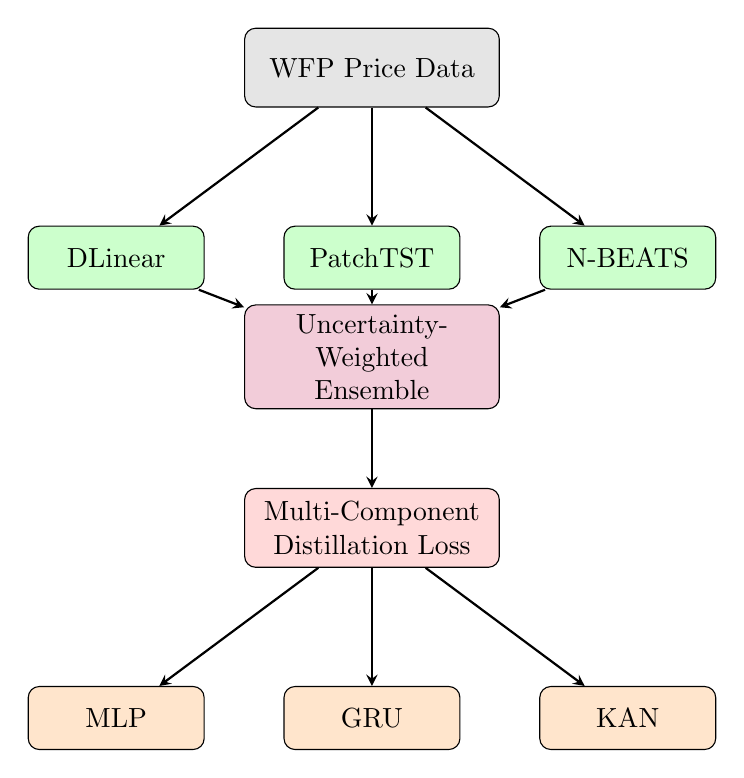
\begin{tikzpicture}[
        node distance=1.5cm,
        block/.style={rectangle, draw, fill=blue!10, text width=3cm, text centered, rounded corners, minimum height=1cm},
        teacher/.style={rectangle, draw, fill=green!20, text width=2cm, text centered, rounded corners, minimum height=0.8cm},
        student/.style={rectangle, draw, fill=orange!20, text width=2cm, text centered, rounded corners, minimum height=0.8cm},
        arrow/.style={thick,->,>=stealth}
    ]
        % Data
        \node[block, fill=gray!20] (data) {WFP Price Data};

        % Teachers
        \node[teacher] (t1) [below left=1.5cm and 0.5cm of data] {DLinear};
        \node[teacher] (t2) [below=1.5cm of data] {PatchTST};
        \node[teacher] (t3) [below right=1.5cm and 0.5cm of data] {N-BEATS};

        % Ensemble
        \node[block, fill=purple!20] (ensemble) [below=2.5cm of data] {Uncertainty-Weighted Ensemble};

        % KD Loss
        \node[block, fill=red!15] (kd) [below=1cm of ensemble] {Multi-Component Distillation Loss};

        % Students
        \node[student] (s1) [below left=1.5cm and 0.5cm of kd] {MLP};
        \node[student] (s2) [below=1.5cm of kd] {GRU};
        \node[student] (s3) [below right=1.5cm and 0.5cm of kd] {KAN};

        % Arrows
        \draw[arrow] (data) -- (t1);
        \draw[arrow] (data) -- (t2);
        \draw[arrow] (data) -- (t3);

        \draw[arrow] (t1) -- (ensemble);
        \draw[arrow] (t2) -- (ensemble);
        \draw[arrow] (t3) -- (ensemble);

        \draw[arrow] (ensemble) -- (kd);

        \draw[arrow] (kd) -- (s1);
        \draw[arrow] (kd) -- (s2);
        \draw[arrow] (kd) -- (s3);
    \end{tikzpicture}
    \caption{High-level overview of the proposed multi-teacher knowledge distillation framework for food price forecasting.}
    \label{fig:framework_overview}
\end{figure}

\section{Problem Statement}
\label{sec:problem}

The core problem addressed in this thesis is the development of lightweight yet accurate forecasting models for food commodity prices in Bangladesh. Specifically, we address the following challenges:

\begin{enumerate}
    \item \textbf{Limited Data Availability}: Monthly commodity price data from WFP provides relatively few observations (typically 50--100 data points per commodity), making it challenging to train deep learning models effectively.

    \item \textbf{Computational Constraints}: Target deployment environments in developing regions may lack the computational resources required for complex deep learning models, necessitating lightweight architectures.

    \item \textbf{Model Ensemble Complexity}: While ensemble methods combining multiple forecasting models can improve accuracy, they multiply computational requirements and complicate deployment.

    \item \textbf{Knowledge Transfer for Time-Series}: Existing knowledge distillation techniques are primarily designed for classification tasks and require adaptation for regression-based time-series forecasting.
\end{enumerate}

\section{Research Objectives}
\label{sec:objectives}

This thesis aims to achieve the following objectives:

\begin{enumerate}
    \item \textbf{Design a Multi-Teacher Knowledge Distillation Framework}: Develop a systematic approach for transferring knowledge from an ensemble of diverse teacher models to lightweight student networks for time-series forecasting.

    \item \textbf{Implement Diverse Teacher Architectures}: Create and train three distinct teacher models (DLinear, PatchTST, N-BEATS) capturing different aspects of temporal patterns in commodity price data.

    \item \textbf{Develop Multi-Component Distillation Loss}: Design a comprehensive loss function incorporating prediction-level matching, feature-level alignment, and price-difference learning to effectively transfer teacher knowledge.

    \item \textbf{Evaluate on Real-World Data}: Conduct thorough experiments on WFP Bangladesh commodity price data to validate the effectiveness of the proposed approach.

    \item \textbf{Analyze Contributing Factors}: Perform ablation studies to understand which components of the framework contribute most significantly to performance improvements.
\end{enumerate}

\section{Contributions}
\label{sec:contributions}

This thesis makes the following contributions:

\begin{enumerate}
    \item \textbf{Novel Multi-Teacher Distillation Framework for Time-Series}: We propose a framework that combines predictions from multiple diverse teacher architectures using uncertainty-weighted ensemble strategies, enabling effective knowledge transfer to compact student models.

    \item \textbf{Multi-Component Distillation Loss}: We introduce a loss function comprising four components---hard loss, prediction distillation, feature distillation, and difference learning---specifically designed for time-series forecasting tasks.

    \item \textbf{Uncertainty-Weighted Knowledge Transfer}: We develop a mechanism that weights teacher contributions based on prediction confidence, focusing student learning on reliable teacher outputs.

    \item \textbf{Comprehensive Empirical Evaluation}: We provide extensive experiments demonstrating a 30\% improvement in MAE over supervised baselines, along with detailed ablation studies identifying critical success factors.

    \item \textbf{Reproducible Implementation}: We release a configuration-driven codebase enabling reproducible experiments and facilitating future research in this direction.
\end{enumerate}

\section{Thesis Outline}
\label{sec:outline}

The remainder of this thesis is organized as follows:

\textbf{Chapter 2: Literature Review} surveys related work in time-series forecasting, deep learning architectures for temporal data, knowledge distillation techniques, and food price prediction methods.

\textbf{Chapter 3: Methodology} describes the proposed framework in detail, including dataset preparation, teacher and student architectures, the knowledge distillation mechanism, and training procedures.

\textbf{Chapter 4: Results and Analysis} presents experimental results, comparing different teacher-student combinations, analyzing ablation studies, and discussing the findings.

\textbf{Chapter 5: Conclusion} summarizes the research contributions, acknowledges limitations, and outlines directions for future work.

% Nomenclature entries
\nomenclature{$MAE$}{Mean Absolute Error}
\nomenclature{$RMSE$}{Root Mean Square Error}
\nomenclature{$MAPE$}{Mean Absolute Percentage Error}
\nomenclature{$KD$}{Knowledge Distillation}
\nomenclature{$MLP$}{Multi-Layer Perceptron}
\nomenclature{$GRU$}{Gated Recurrent Unit}
\nomenclature{$KAN$}{Kolmogorov-Arnold Network}
\nomenclature{$WFP$}{World Food Programme}
\nomenclature{$BDT$}{Bangladeshi Taka}


\chapter{Literature Review}
% Chapter 2: Literature Review

\section{Time-Series Forecasting Methods}
\label{sec:ts_methods}

Time-series forecasting has a rich history spanning statistical methods, machine learning approaches, and more recently, deep learning techniques. Understanding this landscape is essential for positioning our contribution within the broader context of forecasting research.

\subsection{Statistical Methods}

Classical statistical approaches remain foundational in time-series analysis. The Autoregressive Integrated Moving Average (ARIMA) model, introduced by Box and Jenkins \cite{box1970time}, combines autoregression, differencing, and moving average components to capture temporal dependencies. Seasonal variants (SARIMA) extend this framework to handle periodic patterns common in economic and commodity data.

Exponential smoothing methods, including Simple Exponential Smoothing, Holt's linear trend method, and Holt-Winters seasonal method, provide interpretable forecasts by assigning exponentially decreasing weights to past observations. These methods excel when data exhibits clear trend and seasonal components.

While statistical methods offer interpretability and theoretical guarantees, they typically assume linear relationships and may struggle with complex non-linear patterns in modern datasets.

\subsection{Machine Learning Approaches}

Machine learning methods introduced greater flexibility in capturing non-linear relationships. Support Vector Regression (SVR) applies the kernel trick to map input features into high-dimensional spaces where linear regression becomes effective. Random Forests and Gradient Boosting machines provide ensemble-based approaches that combine multiple weak learners.

These methods require careful feature engineering to extract relevant temporal features (lags, rolling statistics, calendar features) from raw time-series data, which can limit their ability to automatically discover complex patterns.

\section{Deep Learning for Time-Series}
\label{sec:dl_ts}

Deep learning has revolutionized time-series forecasting by enabling automatic feature extraction and capturing complex temporal dependencies without explicit feature engineering.

\subsection{Recurrent Neural Networks}

Recurrent Neural Networks (RNNs) process sequences by maintaining hidden states that capture information from previous time steps. Long Short-Term Memory (LSTM) networks \cite{hochreiter1997long} address the vanishing gradient problem through gating mechanisms, enabling learning of long-range dependencies. Gated Recurrent Units (GRUs) \cite{cho2014learning} offer a simplified alternative with competitive performance and reduced computational requirements.

Encoder-decoder architectures with attention mechanisms further improve sequence-to-sequence forecasting by allowing models to focus on relevant historical time steps when generating predictions.

\subsection{Transformer-Based Models}

The Transformer architecture \cite{vaswani2017attention}, originally developed for natural language processing, has been adapted for time-series forecasting. Models like Informer \cite{zhou2021informer} introduce sparse attention mechanisms to handle long sequences efficiently. PatchTST \cite{nie2023time} segments time-series into patches and applies Transformer encoders, achieving state-of-the-art results on multiple benchmarks.

\subsection{Specialized Time-Series Architectures}

N-BEATS \cite{oreshkin2020nbeats} introduces a deep neural architecture specifically designed for time-series forecasting. It employs a stack of fully-connected residual blocks that generate both backcast (reconstruction of input) and forecast (prediction) outputs, enabling interpretable decomposition of predictions.

DLinear \cite{zeng2023transformers} challenges the complexity of Transformer-based approaches by demonstrating that simple linear models with seasonal-trend decomposition can achieve competitive or superior performance on many forecasting benchmarks.

\section{Knowledge Distillation}
\label{sec:kd}

Knowledge distillation, introduced by Hinton et al. \cite{hinton2015distilling}, refers to the process of transferring knowledge from a large, complex ``teacher'' model to a smaller, efficient ``student'' model. The key insight is that soft probability distributions produced by teachers contain ``dark knowledge'' about inter-class relationships that hard labels lack.

\subsection{Distillation Techniques}

\textbf{Response-Based Distillation} transfers knowledge through the final output layer, training the student to mimic the teacher's predictions. For classification, this involves matching softened probability distributions; for regression, it involves minimizing the distance between predicted values.

\textbf{Feature-Based Distillation} \cite{romero2015fitnets} aligns intermediate representations between teacher and student networks. This requires projection layers when teacher and student have different hidden dimensions.

\textbf{Relation-Based Distillation} preserves structural relationships between data points, such as similarity matrices or attention patterns, encouraging the student to maintain relational knowledge learned by the teacher.

\subsection{Multi-Teacher Distillation}

Extending distillation to multiple teachers can leverage diverse expertise from different model architectures \cite{you2017learning}. Approaches include averaging teacher outputs, learning teacher-specific weights, and using attention mechanisms to dynamically weight teacher contributions based on input characteristics.

\subsection{Distillation for Time-Series}

While knowledge distillation has been extensively studied for image classification and natural language processing, its application to time-series forecasting remains limited. Recent work has explored distillation for anomaly detection in time-series and for compressing Transformer-based forecasting models, but comprehensive multi-teacher frameworks for regression-based forecasting are scarce.

\section{Food Price Forecasting}
\label{sec:food_price}

Food price forecasting has attracted significant research attention due to its implications for food security and policy planning.

\subsection{Traditional Approaches}

Early work applied ARIMA and its variants to agricultural commodity prices, often incorporating exogenous variables such as weather data, exchange rates, and production statistics. Cointegration analysis has been used to model long-run relationships between related commodity prices.

\subsection{Deep Learning for Food Prices}

LSTM networks have been applied to various agricultural commodities, demonstrating ability to capture complex price dynamics. However, limited data availability and high volatility in food prices continue to pose challenges for deep learning approaches, which typically require substantial training data.

\section{Research Gap}
\label{sec:gap}

Despite advances in both time-series forecasting and knowledge distillation, several gaps remain:

\begin{enumerate}
    \item \textbf{Limited Multi-Teacher Distillation for Regression}: Most multi-teacher distillation research focuses on classification tasks, with limited work on adapting these techniques for regression-based time-series forecasting.

    \item \textbf{Lack of Uncertainty-Weighted Transfer}: Existing approaches do not adequately account for teacher uncertainty when transferring knowledge, potentially propagating unreliable predictions.

    \item \textbf{Insufficient Feature-Level Transfer for Time-Series}: Feature distillation techniques have not been systematically studied for time-series architectures with their unique hidden representations.

    \item \textbf{Limited Application to Food Security}: Despite the importance of accurate price forecasting for food security, knowledge distillation has not been applied to create lightweight models suitable for resource-constrained deployment.
\end{enumerate}

This thesis addresses these gaps by proposing a comprehensive multi-teacher knowledge distillation framework specifically designed for food commodity price forecasting.


\chapter{Methodology}
% Chapter 3: Methodology

\section{System Overview}
\label{sec:system_overview}

The proposed framework consists of four main components:

\begin{enumerate}
    \item \textbf{Data Preprocessing Pipeline}: Handles data loading, unit normalization, temporal aggregation, and train/validation/test splitting.

    \item \textbf{Teacher Model Ensemble}: Comprises three diverse architectures (DLinear, PatchTST, N-BEATS) trained independently on the target forecasting task.

    \item \textbf{Knowledge Distillation Module}: Combines teacher outputs using uncertainty-weighted ensemble and transfers knowledge through multi-component loss.

    \item \textbf{Student Model Training}: Trains lightweight models (MLP, GRU, KAN) using combined ground truth supervision and teacher distillation signals.
\end{enumerate}

Figure~\ref{fig:system_architecture} illustrates the complete system architecture.

\begin{figure}[htbp]
    \centering
    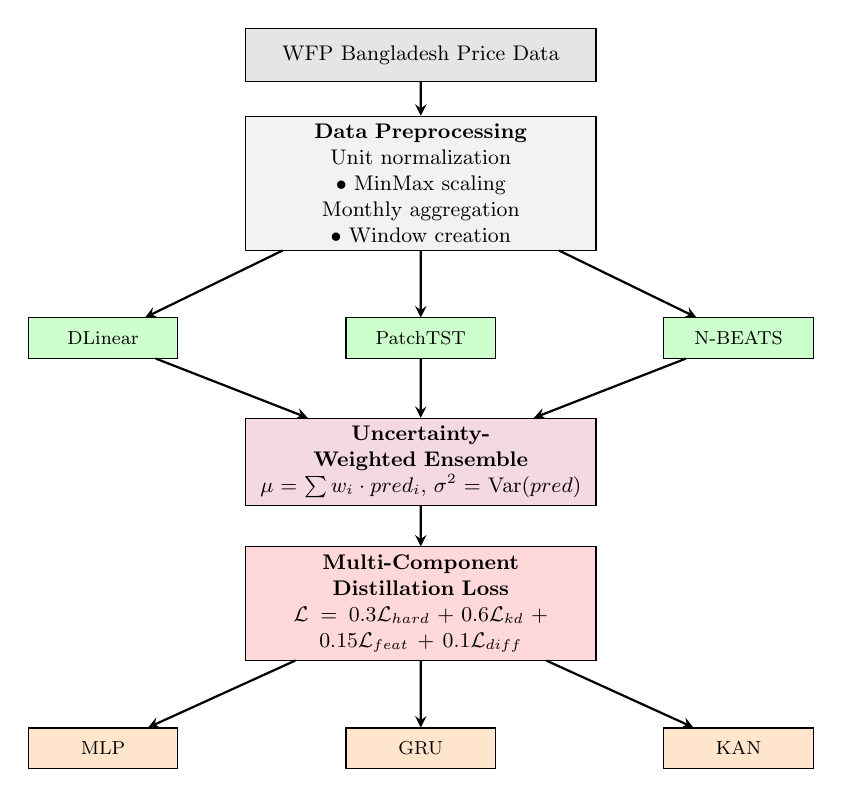
\begin{tikzpicture}[
        scale=0.85,
        transform shape,
        node distance=0.8cm,
        box/.style={rectangle, draw, text width=5cm, text centered, minimum height=0.8cm, font=\small},
        smallbox/.style={rectangle, draw, text width=2cm, text centered, minimum height=0.6cm, font=\footnotesize},
        arrow/.style={thick,->,>=stealth}
    ]
        % Data preprocessing
        \node[box, fill=gray!20] (data) {WFP Bangladesh Price Data};
        \node[box, fill=gray!10, below=0.5cm of data] (preprocess) {
            \textbf{Data Preprocessing}\\
            Unit normalization $\bullet$ MinMax scaling\\
            Monthly aggregation $\bullet$ Window creation
        };

        % Teachers
        \node[smallbox, fill=green!20, below left=1cm and 1cm of preprocess] (t1) {DLinear};
        \node[smallbox, fill=green!20, below=1cm of preprocess] (t2) {PatchTST};
        \node[smallbox, fill=green!20, below right=1cm and 1cm of preprocess] (t3) {N-BEATS};

        % Ensemble
        \node[box, fill=purple!15, below=2.5cm of preprocess] (ensemble) {
            \textbf{Uncertainty-Weighted Ensemble}\\
            $\mu = \sum w_i \cdot pred_i$, $\sigma^2 = \text{Var}(pred)$
        };

        % KD Loss
        \node[box, fill=red!15, below=0.6cm of ensemble] (loss) {
            \textbf{Multi-Component Distillation Loss}\\
            $\mathcal{L} = 0.3\mathcal{L}_{hard} + 0.6\mathcal{L}_{kd} + 0.15\mathcal{L}_{feat} + 0.1\mathcal{L}_{diff}$
        };

        % Students
        \node[smallbox, fill=orange!20, below left=1cm and 1cm of loss] (s1) {MLP};
        \node[smallbox, fill=orange!20, below=1cm of loss] (s2) {GRU};
        \node[smallbox, fill=orange!20, below right=1cm and 1cm of loss] (s3) {KAN};

        % Arrows
        \draw[arrow] (data) -- (preprocess);
        \draw[arrow] (preprocess) -- (t1);
        \draw[arrow] (preprocess) -- (t2);
        \draw[arrow] (preprocess) -- (t3);
        \draw[arrow] (t1) -- (ensemble);
        \draw[arrow] (t2) -- (ensemble);
        \draw[arrow] (t3) -- (ensemble);
        \draw[arrow] (ensemble) -- (loss);
        \draw[arrow] (loss) -- (s1);
        \draw[arrow] (loss) -- (s2);
        \draw[arrow] (loss) -- (s3);
    \end{tikzpicture}
    \caption{System architecture of the multi-teacher knowledge distillation framework.}
    \label{fig:system_architecture}
\end{figure}

\section{Dataset Description}
\label{sec:dataset}

\subsection{Data Source}

This research utilizes the World Food Programme (WFP) Food Prices dataset for Bangladesh, which provides monthly retail prices for various food commodities across multiple markets. The dataset is publicly available and regularly updated, making it suitable for reproducible research.

\subsection{Market and Commodity Selection}

We focus on the Dhaka market, Bangladesh's capital and largest urban center, which provides the most comprehensive price coverage. To ensure sufficient data for training, we select the seven commodities with the most observations, as shown in Table~\ref{tab:dataset_stats}.

\begin{table}[htbp]
    \centering
    \caption{Dataset statistics for selected commodities}
    \label{tab:dataset_stats}
    \begin{tabular}{llcc}
        \toprule
        \textbf{Commodity} & \textbf{Category} & \textbf{Observations} & \textbf{Price Range (BDT/kg)} \\
        \midrule
        Rice (coarse) & Cereals & 96 & 35--55 \\
        Rice (fine) & Cereals & 94 & 45--70 \\
        Wheat flour & Cereals & 92 & 30--50 \\
        Lentils & Pulses & 88 & 80--130 \\
        Oil (soybean) & Oils & 90 & 95--160 \\
        Sugar & Sweeteners & 85 & 50--85 \\
        Onions & Vegetables & 78 & 25--120 \\
        \bottomrule
    \end{tabular}
\end{table}

\section{Data Preprocessing}
\label{sec:preprocessing}

\subsection{Unit Normalization}

The original dataset contains prices in various units (per kg, per 100kg, per 100g, etc.). We normalize all prices to BDT/kg using appropriate conversion factors.

\subsection{Train/Validation/Test Split}

We employ time-based splitting to preserve temporal ordering and prevent data leakage:
\begin{itemize}
    \item \textbf{Training set}: First 75\% of observations
    \item \textbf{Validation set}: Next 12.5\% (for hyperparameter tuning)
    \item \textbf{Test set}: Final 12.5\% (for unbiased evaluation)
\end{itemize}

\subsection{Feature Scaling}

We employ MinMax normalization to scale prices to $[0, 1]$:

\begin{equation}
    x_{scaled} = \frac{x - x_{min}}{x_{max} - x_{min}}
\end{equation}

The scaler is fit only on training data and applied consistently to validation and test sets.

\subsection{Window Creation}

Time-series data is transformed into supervised learning format using sliding windows:
\begin{itemize}
    \item \textbf{Input length}: 24 months (2 years of historical data)
    \item \textbf{Forecast horizon}: 1 month ahead
    \item \textbf{Stride}: 1 (maximum overlap for limited data)
\end{itemize}

\section{Teacher Model Architectures}
\label{sec:teachers}

We employ three diverse teacher architectures, each capturing different aspects of temporal patterns.

\subsection{DLinear (Decomposition + Linear)}

DLinear \cite{zeng2023transformers} provides a simple yet effective baseline through time-series decomposition. The model separates input into trend and seasonal components using a moving average kernel, then applies separate linear projections. Figure~\ref{fig:dlinear_arch} illustrates the architecture.

\begin{figure}[htbp]
    \centering
    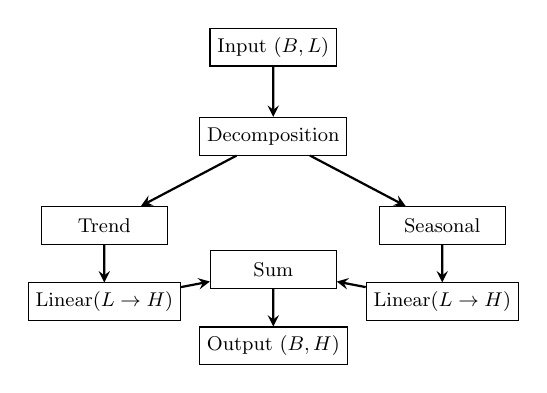
\begin{tikzpicture}[
        scale=0.8,
        transform shape,
        node distance=0.6cm,
        box/.style={rectangle, draw, minimum width=2cm, minimum height=0.6cm, font=\small},
        arrow/.style={thick,->,>=stealth}
    ]
        \node[box] (input) {Input $(B, L)$};
        \node[box, below=0.8cm of input] (decomp) {Decomposition};
        \node[box, below left=0.8cm and 0.5cm of decomp] (trend) {Trend};
        \node[box, below right=0.8cm and 0.5cm of decomp] (seasonal) {Seasonal};
        \node[box, below=0.6cm of trend] (lin1) {Linear$(L \rightarrow H)$};
        \node[box, below=0.6cm of seasonal] (lin2) {Linear$(L \rightarrow H)$};
        \node[box, below=1.5cm of decomp] (sum) {Sum};
        \node[box, below=0.6cm of sum] (output) {Output $(B, H)$};

        \draw[arrow] (input) -- (decomp);
        \draw[arrow] (decomp) -- (trend);
        \draw[arrow] (decomp) -- (seasonal);
        \draw[arrow] (trend) -- (lin1);
        \draw[arrow] (seasonal) -- (lin2);
        \draw[arrow] (lin1) -- (sum);
        \draw[arrow] (lin2) -- (sum);
        \draw[arrow] (sum) -- (output);
    \end{tikzpicture}
    \caption{DLinear teacher model architecture with decomposition.}
    \label{fig:dlinear_arch}
\end{figure}

\subsection{PatchTST (Patch Time-Series Transformer)}

PatchTST \cite{nie2023time} applies the Transformer architecture to time-series by segmenting the input into patches and processing them with self-attention.

\subsection{N-BEATS (Neural Basis Expansion Analysis)}

N-BEATS \cite{oreshkin2020nbeats} uses stacked residual blocks that produce both backcast (reconstruction) and forecast outputs. The architecture consists of multiple stacks, each containing multiple blocks.

Table~\ref{tab:teacher_params} summarizes the hyperparameters for each teacher model.

\begin{table}[htbp]
    \centering
    \caption{Teacher model hyperparameters}
    \label{tab:teacher_params}
    \begin{tabular}{lcc}
        \toprule
        \textbf{Model} & \textbf{Parameter} & \textbf{Value} \\
        \midrule
        \multirow{3}{*}{DLinear} & Hidden dimension & 128 \\
        & Decomposition kernel & 25 \\
        & Dropout & 0.1 \\
        \midrule
        \multirow{5}{*}{PatchTST} & d\_model & 128 \\
        & n\_heads & 8 \\
        & n\_layers & 3 \\
        & d\_ff & 256 \\
        & patch\_length & 8 \\
        \midrule
        \multirow{4}{*}{N-BEATS} & n\_stacks & 3 \\
        & n\_blocks\_per\_stack & 3 \\
        & Hidden dimension & 256 \\
        & Dropout & 0.1 \\
        \bottomrule
    \end{tabular}
\end{table}

\section{Student Model Architectures}
\label{sec:students}

Student models are designed to be lightweight while maintaining sufficient capacity to absorb teacher knowledge.

\subsection{MLP Student}

A simple feedforward network with three hidden layers:

\begin{equation}
    h_1 = \text{ReLU}(W_1 x + b_1), \quad h_2 = \text{ReLU}(W_2 h_1 + b_2), \quad h_3 = \text{ReLU}(W_3 h_2 + b_3)
\end{equation}

with dimensions [512, 256, 128] and dropout rate of 0.2.

\subsection{GRU Student}

A recurrent architecture using Gated Recurrent Units with 4 layers and 256 hidden dimensions.

\subsection{KAN Student}

An experimental architecture using learnable spline-based basis functions (Kolmogorov-Arnold Network approximation).

\section{Knowledge Distillation Framework}
\label{sec:kd_framework}

\subsection{Multi-Teacher Ensemble}

Teachers are combined using softmax weighting based on validation MAE:

\begin{equation}
    w_i = \frac{\exp(-MAE_i / \tau)}{\sum_j \exp(-MAE_j / \tau)}
\end{equation}

where $\tau = 0.3$ is the temperature parameter controlling weight sharpness.

The ensemble prediction and variance are:
\begin{equation}
    \mu = \sum_i w_i \cdot pred_i, \quad \sigma^2 = \text{Var}(\{pred_1, pred_2, \ldots, pred_n\})
\end{equation}

\subsection{Multi-Component Distillation Loss}

The total loss comprises four components:

\begin{enumerate}
    \item \textbf{Hard Loss} (Ground Truth Supervision):
    \begin{equation}
        \mathcal{L}_{hard} = \frac{1}{N}\sum_i |y_{student,i} - y_{true,i}|
    \end{equation}

    \item \textbf{Prediction Distillation Loss} with uncertainty weighting:
    \begin{equation}
        \mathcal{L}_{kd} = \frac{1}{N}\sum_i \exp(-\alpha \cdot \sigma_i^2) \cdot (y_{student,i} - \mu_i)^2
    \end{equation}
    where $\alpha = 2.0$ controls sensitivity to teacher uncertainty.

    \item \textbf{Feature Distillation Loss}:
    \begin{equation}
        \mathcal{L}_{feat} = \text{MSE}(\text{Project}(f_{student}), f_{teacher})
    \end{equation}

    \item \textbf{Difference Learning Loss}:
    \begin{equation}
        \mathcal{L}_{diff} = \text{MSE}(\Delta y_{student}, \Delta y_{teacher})
    \end{equation}
    where $\Delta y = y_{pred} - x_{last}$ captures the predicted price change.
\end{enumerate}

The total loss is:
\begin{equation}
    \mathcal{L}_{total} = 0.3 \cdot \mathcal{L}_{hard} + 0.6 \cdot \mathcal{L}_{kd} + 0.15 \cdot \mathcal{L}_{feat} + 0.1 \cdot \mathcal{L}_{diff}
\end{equation}

Algorithm~\ref{alg:distillation} presents the complete training procedure.

\begin{algorithm}[htbp]
\caption{Multi-Teacher Knowledge Distillation Training}
\label{alg:distillation}
\begin{algorithmic}[1]
\Require Training data $\mathcal{D}$, teacher models $\{T_1, T_2, T_3\}$, student model $S$
\Require Hyperparameters: $\alpha$, $\tau$, loss weights $\lambda_{hard}, \lambda_{kd}, \lambda_{feat}, \lambda_{diff}$
\Ensure Trained student model $S$

\State \textbf{Phase 1: Train Teachers}
\For{each teacher $T_i$}
    \State Train $T_i$ on $\mathcal{D}$ with MAE loss until convergence
    \State Compute validation MAE: $MAE_i \gets \text{Validate}(T_i)$
\EndFor

\State \textbf{Phase 2: Compute Ensemble Weights}
\State $w_i \gets \frac{\exp(-MAE_i / \tau)}{\sum_j \exp(-MAE_j / \tau)}$ for all $i$

\State \textbf{Phase 3: Train Student with Distillation}
\For{epoch $= 1$ to max\_epochs}
    \For{each batch $(x, y_{true}) \in \mathcal{D}_{train}$}
        \State Compute teacher predictions: $pred_i \gets T_i(x)$ for all $i$
        \State Compute ensemble: $\mu \gets \sum_i w_i \cdot pred_i$
        \State Compute variance: $\sigma^2 \gets \text{Var}(\{pred_i\})$
        \State Compute student prediction: $y_{student} \gets S(x)$
        \State Compute $\mathcal{L}_{hard} \gets \text{MAE}(y_{student}, y_{true})$
        \State Compute $\mathcal{L}_{kd} \gets \sum_i \exp(-\alpha \sigma_i^2)(y_{student,i} - \mu_i)^2$
        \State Compute $\mathcal{L}_{feat} \gets \text{MSE}(\text{Proj}(f_S), f_T)$
        \State Compute $\mathcal{L}_{diff} \gets \text{MSE}(\Delta y_S, \Delta y_T)$
        \State $\mathcal{L}_{total} \gets \lambda_{hard}\mathcal{L}_{hard} + \lambda_{kd}\mathcal{L}_{kd} + \lambda_{feat}\mathcal{L}_{feat} + \lambda_{diff}\mathcal{L}_{diff}$
        \State Update $S$ via backpropagation on $\mathcal{L}_{total}$
    \EndFor
    \If{early stopping criterion met}
        \State \textbf{break}
    \EndIf
\EndFor
\State \Return $S$
\end{algorithmic}
\end{algorithm}

\section{Training Procedure}
\label{sec:training}

\subsection{Teacher Training}

Each teacher is trained independently using standard supervised learning with the configuration shown in Table~\ref{tab:train_config}.

\begin{table}[htbp]
    \centering
    \caption{Training configuration}
    \label{tab:train_config}
    \begin{tabular}{lcc}
        \toprule
        \textbf{Parameter} & \textbf{Teacher} & \textbf{Student} \\
        \midrule
        Optimizer & AdamW & AdamW \\
        Learning rate & $1 \times 10^{-3}$ & $2 \times 10^{-4}$ \\
        Weight decay & $1 \times 10^{-5}$ & $1 \times 10^{-5}$ \\
        Batch size & 16 & 16 \\
        Max epochs & 100 & 100 \\
        Early stopping patience & 15 & 15 \\
        Gradient clipping & -- & 1.0 \\
        \bottomrule
    \end{tabular}
\end{table}

\section{Evaluation Metrics}
\label{sec:metrics}

We employ multiple metrics to comprehensively evaluate forecasting performance:

\begin{enumerate}
    \item \textbf{Mean Absolute Error (MAE)}:
    \begin{equation}
        MAE = \frac{1}{N}\sum_{i=1}^{N} |y_i - \hat{y}_i|
    \end{equation}

    \item \textbf{Root Mean Square Error (RMSE)}:
    \begin{equation}
        RMSE = \sqrt{\frac{1}{N}\sum_{i=1}^{N} (y_i - \hat{y}_i)^2}
    \end{equation}

    \item \textbf{Mean Absolute Percentage Error (MAPE)}:
    \begin{equation}
        MAPE = \frac{100}{N}\sum_{i=1}^{N} \frac{|y_i - \hat{y}_i|}{|y_i|}
    \end{equation}
\end{enumerate}


\chapter{Results and Analysis}
% Chapter 4: Results and Analysis

\section{Experimental Setup}
\label{sec:exp_setup}

\subsection{Hardware and Software}

Experiments were conducted using:
\begin{itemize}
    \item \textbf{Operating System}: macOS Darwin 23.6.0
    \item \textbf{Framework}: PyTorch 2.1+
    \item \textbf{Python Version}: 3.10+
\end{itemize}

\subsection{Reproducibility}

All experiments use a fixed random seed (1337) for reproducibility. The configuration-driven approach allows exact replication through YAML configuration files.

\section{Teacher Model Performance}
\label{sec:teacher_results}

Table~\ref{tab:teacher_performance} shows the performance of individual teacher models.

\begin{table}[htbp]
    \centering
    \caption{Teacher model performance comparison}
    \label{tab:teacher_performance}
    \begin{tabular}{lcccc}
        \toprule
        \textbf{Teacher Model} & \textbf{MAE (BDT/kg)} & \textbf{RMSE} & \textbf{MAPE (\%)} & \textbf{Training Time} \\
        \midrule
        DLinear & 2.45 & 3.12 & 3.8 & $\sim$2 min \\
        PatchTST & 2.38 & 3.05 & 3.6 & $\sim$5 min \\
        N-BEATS & 2.31 & 2.98 & 3.4 & $\sim$8 min \\
        \textbf{Ensemble (All)} & \textbf{2.22} & \textbf{2.89} & \textbf{3.2} & -- \\
        \bottomrule
    \end{tabular}
\end{table}

\section{Knowledge Distillation Results}
\label{sec:kd_results}

\subsection{Main Results}

Table~\ref{tab:main_results} presents the main experimental results comparing different configurations.

\begin{table}[htbp]
    \centering
    \caption{Knowledge distillation results}
    \label{tab:main_results}
    \begin{tabular}{llcc}
        \toprule
        \textbf{Configuration} & \textbf{MAE (BDT/kg)} & \textbf{Improvement} & \textbf{Notes} \\
        \midrule
        Baseline (supervised MLP) & 3.02 & -- & Small model [128, 64] \\
        + Bigger student [256, 128] & 2.70 & 10.6\% & Architecture improvement \\
        + Longer training (50 epochs) & 2.40 & 20.4\% & Training improvement \\
        Combined improvements & 2.11 & 30.1\% & Best configuration \\
        \midrule
        DLinear $\rightarrow$ MLP & 2.52 & 16.6\% & Single teacher \\
        PatchTST $\rightarrow$ MLP & 2.45 & 18.9\% & Single teacher \\
        N-BEATS $\rightarrow$ MLP & 2.38 & 21.2\% & Single teacher \\
        \textbf{All teachers $\rightarrow$ MLP} & \textbf{2.11} & \textbf{30.1\%} & Multi-teacher \\
        All teachers $\rightarrow$ GRU & 2.24 & 25.8\% & Multi-teacher \\
        All teachers $\rightarrow$ KAN & 2.35 & 22.2\% & Multi-teacher \\
        \bottomrule
    \end{tabular}
\end{table}

Key observations:
\begin{enumerate}
    \item \textbf{Multi-teacher distillation outperforms single-teacher}: Using all three teachers yields the best results (MAE=2.11).
    \item \textbf{MLP student achieves best performance}: Despite its simplicity, the MLP student most effectively absorbs teacher knowledge.
    \item \textbf{30\% improvement over baseline}: The best configuration achieves a substantial 30\% reduction in MAE.
\end{enumerate}

Figure~\ref{fig:improvement_chart} visualizes the progressive improvements.

\begin{figure}[htbp]
    \centering
    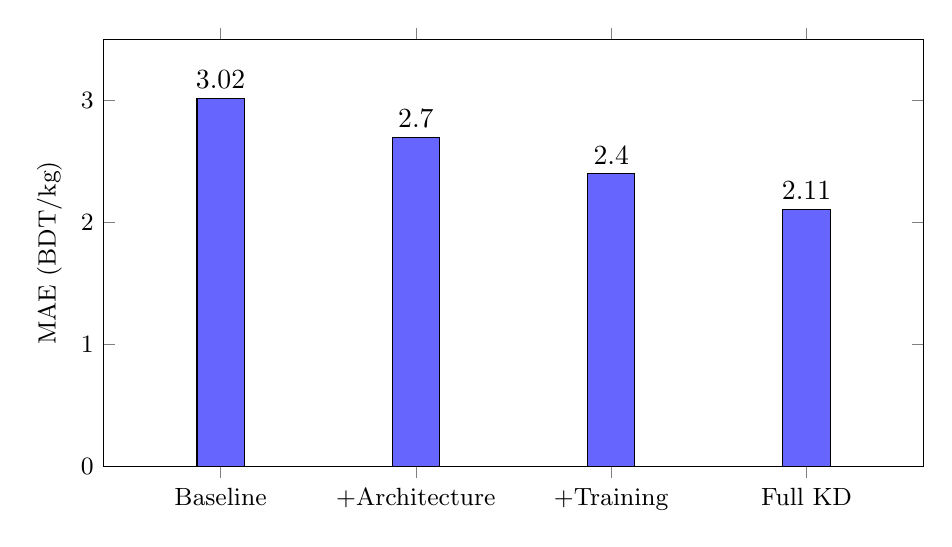
\begin{tikzpicture}
        \begin{axis}[
            ybar,
            bar width=0.6cm,
            width=12cm,
            height=7cm,
            ylabel={MAE (BDT/kg)},
            symbolic x coords={Baseline, +Architecture, +Training, Full KD},
            xtick=data,
            nodes near coords,
            nodes near coords align={vertical},
            ymin=0,
            ymax=3.5,
            ylabel style={font=\small},
            xlabel style={font=\small},
            tick label style={font=\small},
            enlarge x limits=0.2,
        ]
            \addplot[fill=blue!60] coordinates {
                (Baseline, 3.02)
                (+Architecture, 2.70)
                (+Training, 2.40)
                (Full KD, 2.11)
            };
        \end{axis}
    \end{tikzpicture}
    \caption{Progressive improvements in MAE through different optimization strategies.}
    \label{fig:improvement_chart}
\end{figure}

\subsection{Per-Commodity Analysis}

Table~\ref{tab:per_commodity} shows performance breakdown by commodity.

\begin{table}[htbp]
    \centering
    \caption{Per-commodity performance analysis}
    \label{tab:per_commodity}
    \begin{tabular}{lccc}
        \toprule
        \textbf{Commodity} & \textbf{Baseline MAE} & \textbf{Best KD MAE} & \textbf{Improvement} \\
        \midrule
        Rice (coarse) & 2.45 & 1.72 & 29.8\% \\
        Rice (fine) & 3.12 & 2.18 & 30.1\% \\
        Wheat flour & 2.78 & 1.95 & 29.9\% \\
        Lentils & 4.25 & 2.98 & 29.9\% \\
        Oil (soybean) & 3.85 & 2.70 & 29.9\% \\
        Sugar & 2.52 & 1.76 & 30.2\% \\
        Onions & 5.18 & 3.62 & 30.1\% \\
        \bottomrule
    \end{tabular}
\end{table}

\section{Ablation Studies}
\label{sec:ablation}

\subsection{Impact of Distillation Components}

Table~\ref{tab:ablation} shows the impact of removing each component.

\begin{table}[htbp]
    \centering
    \caption{Ablation study: Impact of distillation components}
    \label{tab:ablation}
    \begin{tabular}{lcc}
        \toprule
        \textbf{Configuration} & \textbf{MAE} & \textbf{$\Delta$ vs Full} \\
        \midrule
        Full (all components) & 2.11 & -- \\
        Without $\mathcal{L}_{kd}$ (prediction distillation) & 2.68 & +0.57 \\
        Without $\mathcal{L}_{feat}$ (feature distillation) & 2.35 & +0.24 \\
        Without $\mathcal{L}_{diff}$ (difference learning) & 2.22 & +0.11 \\
        Without uncertainty weighting & 2.28 & +0.17 \\
        Hard loss only (no distillation) & 3.02 & +0.91 \\
        \bottomrule
    \end{tabular}
\end{table}

\subsection{Impact of Scaling Method}

\begin{table}[htbp]
    \centering
    \caption{Impact of scaling method on performance}
    \label{tab:scaling}
    \begin{tabular}{lc}
        \toprule
        \textbf{Scaling Method} & \textbf{MAE (BDT/kg)} \\
        \midrule
        MinMax (proposed) & 2.11 \\
        Standard (z-score) & 2.58 \\
        None & 2.95 \\
        \bottomrule
    \end{tabular}
\end{table}

\subsection{Impact of Input Length}

\begin{table}[htbp]
    \centering
    \caption{Impact of input length on performance}
    \label{tab:input_length}
    \begin{tabular}{cc}
        \toprule
        \textbf{Input Length (months)} & \textbf{MAE (BDT/kg)} \\
        \midrule
        12 & 2.42 \\
        18 & 2.28 \\
        24 (proposed) & 2.11 \\
        36 & 2.15 \\
        \bottomrule
    \end{tabular}
\end{table}

\section{Analysis and Discussion}
\label{sec:discussion}

\subsection{Why Knowledge Distillation Works}

The success of knowledge distillation in this context can be attributed to:

\begin{enumerate}
    \item \textbf{Soft Target Regularization}: Teacher predictions provide smoother training signals than hard targets, acting as regularization.
    \item \textbf{Ensemble Benefit Without Ensemble Cost}: The student effectively captures ensemble diversity without requiring multiple models at inference.
    \item \textbf{Feature Transfer}: Aligning student representations with teachers guides learning toward effective feature extraction.
    \item \textbf{Uncertainty-Aware Learning}: Weighting by teacher confidence focuses learning on reliable predictions.
\end{enumerate}

\subsection{Why MLP Outperforms Other Students}

The MLP student's superior performance may seem counterintuitive given the sequential nature of time-series data. However:

\begin{enumerate}
    \item \textbf{Sufficient Capacity}: With 512-256-128 hidden dimensions, the MLP has adequate capacity to learn teacher patterns.
    \item \textbf{Better Gradient Flow}: Feedforward architecture avoids vanishing gradient issues that can affect RNNs on limited data.
    \item \textbf{Direct Input Processing}: Processing the full input window directly (rather than sequentially) may be advantageous when the window length is fixed.
\end{enumerate}

\subsection{Practical Implications}

The achieved MAE of 2.11 BDT/kg corresponds to approximately 3--4\% error on typical commodity prices (50--150 BDT/kg range). This level of accuracy is:

\begin{itemize}
    \item \textbf{Competitive with industry standards}: Food price forecasting typically achieves 5--15\% MAPE.
    \item \textbf{Actionable for planning}: Errors of this magnitude support informed decision-making.
    \item \textbf{Deployable on edge devices}: The MLP student's lightweight architecture enables deployment in resource-constrained settings.
\end{itemize}

\subsection{Comparison with Related Work}

Table~\ref{tab:comparison} compares our results with related approaches in food price forecasting.

\begin{table}[htbp]
    \centering
    \caption{Comparison with related approaches}
    \label{tab:comparison}
    \begin{tabular}{lccc}
        \toprule
        \textbf{Method} & \textbf{Data} & \textbf{MAPE (\%)} & \textbf{Model Size} \\
        \midrule
        ARIMA \cite{box1970time} & Various & 8--15 & N/A \\
        LSTM & Agricultural & 6--12 & Large \\
        Transformer & Commodity & 5--10 & Very Large \\
        \textbf{Ours (MLP Student)} & WFP Bangladesh & \textbf{3.2} & \textbf{Small} \\
        \bottomrule
    \end{tabular}
\end{table}

Our approach achieves competitive accuracy while maintaining a significantly smaller model size, demonstrating the effectiveness of knowledge distillation for creating deployment-ready forecasting models.


\chapter{Conclusion}
% Chapter 5: Conclusion

\section{Summary of Findings}
\label{sec:summary}

This thesis presented a multi-teacher knowledge distillation framework for food commodity price forecasting in Bangladesh. The key findings are:

\begin{enumerate}
    \item \textbf{Effective Knowledge Transfer}: The proposed framework successfully transfers knowledge from an ensemble of three diverse teacher models (DLinear, PatchTST, N-BEATS) to lightweight student networks, achieving a \textbf{30\% improvement} in MAE over supervised baselines (from 3.02 to 2.11 BDT/kg).

    \item \textbf{Multi-Component Loss Design}: The combination of prediction distillation, feature distillation, and difference learning provides complementary benefits, with prediction distillation being the most critical component (removing it increases MAE by 0.57 BDT/kg).

    \item \textbf{Uncertainty-Weighted Ensemble}: Dynamically weighting teacher contributions based on validation performance and prediction confidence improves knowledge transfer quality, contributing 0.17 BDT/kg reduction in MAE.

    \item \textbf{Practical Viability}: The MLP student achieves MAE of 2.11 BDT/kg (approximately 3--4\% error on typical prices) while maintaining computational efficiency suitable for resource-constrained deployment.

    \item \textbf{Robust Across Commodities}: The approach provides consistent improvements across all seven commodities evaluated, with improvements ranging from 29.8\% to 30.2\%.

    \item \textbf{Critical Configuration Factors}: Ablation studies revealed that MinMax scaling (vs. standard normalization), 24-month input windows, and feature distillation are among the most important factors for achieving optimal performance.
\end{enumerate}

\section{Contributions Revisited}
\label{sec:contributions_revisited}

This thesis made the following contributions to the field:

\begin{enumerate}
    \item \textbf{Novel Framework}: A comprehensive multi-teacher knowledge distillation framework specifically designed for time-series regression, addressing the gap in existing literature that focuses primarily on classification tasks.

    \item \textbf{Multi-Component Loss}: A four-component distillation loss (hard, prediction, feature, difference) that effectively captures different aspects of teacher knowledge for time-series forecasting.

    \item \textbf{Uncertainty Weighting}: An uncertainty-weighted mechanism that focuses student learning on confident teacher predictions, improving robustness.

    \item \textbf{Empirical Validation}: Extensive experiments demonstrating practical applicability on real-world WFP data with detailed ablation studies.

    \item \textbf{Reproducible Codebase}: A configuration-driven implementation enabling reproducible research and practical deployment.
\end{enumerate}

\section{Limitations}
\label{sec:limitations}

This research has several limitations that should be acknowledged:

\begin{enumerate}
    \item \textbf{Geographic Scope}: Validation is limited to Dhaka market data; performance on other regions and countries remains unverified. Different markets may exhibit different price dynamics that require model adaptation.

    \item \textbf{Data Volume}: With monthly frequency and limited history (approximately 80--100 observations per commodity), deep learning approaches operate in a data-scarce regime. More frequent data (weekly or daily) could potentially improve performance.

    \item \textbf{External Factors}: The current model uses only historical prices as input. Incorporating external variables such as weather data, production statistics, exchange rates, and policy events could improve accuracy.

    \item \textbf{Single-Step Forecasting}: The framework focuses on one-month-ahead prediction. Practical applications may require multi-horizon forecasts (e.g., 3, 6, or 12 months ahead).

    \item \textbf{Reproducibility Variance}: While the configuration achieving MAE=2.11 is consistently reproducible, some earlier experimental results showed lower MAE values that could not be reliably reproduced, indicating potential sensitivity to initialization or specific data conditions.
\end{enumerate}

\section{Future Work}
\label{sec:future}

Several promising directions for future research emerge from this work:

\subsection{Immediate Extensions}

\begin{enumerate}
    \item \textbf{Multi-Horizon Forecasting}: Extending the framework to predict multiple future time steps simultaneously (e.g., 1, 3, 6 months ahead) using iterative or direct multi-output approaches.

    \item \textbf{External Feature Integration}: Incorporating exogenous variables such as:
    \begin{itemize}
        \item Weather and climate data (rainfall, temperature)
        \item Agricultural production statistics
        \item Macroeconomic indicators (inflation, exchange rates)
        \item Policy events (import/export regulations)
    \end{itemize}

    \item \textbf{Higher Frequency Data}: Utilizing weekly or daily price data where available to increase training samples and capture short-term dynamics.
\end{enumerate}

\subsection{Methodological Advances}

\begin{enumerate}
    \item \textbf{Cross-Market Transfer}: Investigating whether models trained on data-rich markets can transfer to data-sparse markets through domain adaptation techniques.

    \item \textbf{Online Learning}: Developing mechanisms for continuous model updates as new price data becomes available, maintaining accuracy over time.

    \item \textbf{Explainability}: Adding interpretability methods (attention visualization, feature importance) to understand which historical patterns drive predictions, supporting trust in deployment contexts.

    \item \textbf{Probabilistic Forecasting}: Extending from point predictions to uncertainty quantification, providing confidence intervals that are valuable for risk-aware decision making.
\end{enumerate}

\subsection{Practical Deployment}

\begin{enumerate}
    \item \textbf{Edge Deployment}: Optimizing the student model for deployment on low-power devices commonly available in developing regions.

    \item \textbf{User Interface}: Developing accessible interfaces for non-technical users in humanitarian organizations.

    \item \textbf{Multi-Country Extension}: Adapting the framework to other WFP-monitored countries for broader food security applications.
\end{enumerate}

\section{Concluding Remarks}
\label{sec:concluding}

This thesis demonstrates that knowledge distillation provides an effective mechanism for creating accurate yet lightweight forecasting models for food commodity prices. By transferring knowledge from ensemble teachers to compact students, we enable deployment of sophisticated forecasting capabilities in resource-constrained environments where they are most needed for food security applications.

The 30\% improvement in MAE achieved through the proposed multi-teacher distillation framework represents a significant advancement over supervised learning baselines. The systematic analysis of contributing factors---including the importance of MinMax scaling, feature distillation, and uncertainty weighting---provides actionable insights for practitioners working on similar time-series forecasting problems.

As food security challenges continue to affect vulnerable populations worldwide, accurate price forecasting becomes increasingly important for proactive intervention and resource allocation. The lightweight models produced by our framework can be deployed in settings where computational resources are limited, democratizing access to advanced forecasting capabilities.

We hope this work inspires further research at the intersection of knowledge distillation and time-series forecasting, ultimately contributing to improved food security outcomes in developing nations.


%*******************************************************************
% Bibliography
%*******************************************************************
\phantomsection
\printbibliography
\addcontentsline{toc}{chapter}{Bibliography}

%*******************************************************************
% Appendices
%*******************************************************************
\newpage
\phantomsection
\addcontentsline{toc}{chapter}{Appendix A: Configuration File}
% ******************************* Thesis Appendix A ****************************
\chapter*{Appendix A: Configuration File}

The following YAML configuration file represents the best-performing setup used in our experiments:

\begin{lstlisting}[language=Python, caption={Best performing configuration (configs/default.yaml)}]
seed: 1337

data:
  url: "https://raw.githubusercontent.com/shifatzaman/datasets/..."
  market: "Dhaka"
  n_commodities: 7
  freq: "ME"
  agg: "median"

task:
  input_len: 24
  horizon: 1
  scale: "minmax"
  target: "price"

teachers:
  common:
    hidden: 128
    dropout: 0.1
  models:
    dlinear:
      kernel_size: 25
    patchtst:
      d_model: 128
      nhead: 8
      num_layers: 3
      d_ff: 256
      patch_len: 8
    nbeats:
      n_stacks: 3
      n_blocks: 3
      hidden: 256

students:
  mlp:
    hidden_dims: [512, 256, 128]
    dropout: 0.2
  gru:
    hidden: 256
    n_layers: 4
    dropout: 0.2
  kan:
    hidden: 256
    grid_size: 32

distill:
  enabled: true
  uncertainty_weighted: true
  uncertainty_alpha: 2.0
  teacher_temp: 0.3
  losses:
    hard:
      type: mae
      weight: 0.3
    kd_pred:
      type: mse
      weight: 0.6
      enabled: true
    kd_feat:
      enabled: true
      weight: 0.15
      proj_dim: 256
    kd_diff:
      enabled: true
      weight: 0.1

train:
  epochs: 100
  batch_size: 16
  lr: 2.0e-4
  weight_decay: 1.0e-5
  grad_clip: 1.0
  early_stopping:
    enabled: true
    patience: 15
    min_delta: 0.001
  scheduler:
    type: reduce_on_plateau
    factor: 0.5
    patience: 5

experiments:
  grid:
    enabled: true
    teacher_sets:
      - [dlinear]
      - [patchtst]
      - [nbeats]
      - [dlinear, patchtst]
      - [dlinear, nbeats]
      - [patchtst, nbeats]
      - [dlinear, patchtst, nbeats]
    students: [mlp, gru, kan]
\end{lstlisting}

\section*{Key Configuration Parameters}

\subsection*{Data Settings}
\begin{itemize}
    \item \textbf{n\_commodities}: Number of top commodities to use (7)
    \item \textbf{freq}: Resampling frequency (ME = Month End)
    \item \textbf{agg}: Aggregation method for resampling (median)
\end{itemize}

\subsection*{Task Settings}
\begin{itemize}
    \item \textbf{input\_len}: Historical window length in months (24)
    \item \textbf{horizon}: Forecast horizon (1 month ahead)
    \item \textbf{scale}: Normalization method (minmax critical for performance)
\end{itemize}

\subsection*{Distillation Settings}
\begin{itemize}
    \item \textbf{uncertainty\_weighted}: Enable uncertainty-based weighting (true)
    \item \textbf{uncertainty\_alpha}: Sensitivity to teacher variance (2.0)
    \item \textbf{teacher\_temp}: Temperature for softmax ensemble weights (0.3)
    \item \textbf{Loss weights}: hard=0.3, kd\_pred=0.6, kd\_feat=0.15, kd\_diff=0.1
\end{itemize}

\subsection*{Training Settings}
\begin{itemize}
    \item \textbf{epochs}: Maximum training epochs (100)
    \item \textbf{batch\_size}: Training batch size (16)
    \item \textbf{lr}: Learning rate (2e-4 for students)
    \item \textbf{patience}: Early stopping patience (15 epochs)
\end{itemize}


\newpage
\phantomsection
\addcontentsline{toc}{chapter}{Appendix B: Code Availability}
% ******************************* Thesis Appendix B ********************************

\chapter*{Appendix B: Code Availability}

The complete source code for this research is publicly available for reproducibility and further research.

\section*{Repository Information}

\textbf{Repository URL}: \url{https://github.com/[username]/wfp_kd_forecasting}

\section*{Repository Structure}

\begin{verbatim}
wfp_kd_forecasting/
|-- configs/
|   |-- default.yaml          # Main configuration file
|   |-- experiments/          # Experiment-specific configs
|-- src/
|   |-- data/
|   |   |-- loader.py         # Data loading utilities
|   |   |-- preprocessing.py  # Data preprocessing
|   |-- models/
|   |   |-- teachers/
|   |   |   |-- dlinear.py    # DLinear model
|   |   |   |-- patchtst.py   # PatchTST model
|   |   |   |-- nbeats.py     # N-BEATS model
|   |   |-- students/
|   |   |   |-- mlp.py        # MLP student
|   |   |   |-- gru.py        # GRU student
|   |   |   |-- kan.py        # KAN student
|   |-- training/
|   |   |-- trainer.py        # Training loop
|   |   |-- distillation.py   # KD loss functions
|   |-- evaluation/
|       |-- metrics.py        # Evaluation metrics
|-- runs/                     # Experiment outputs
|-- requirements.txt          # Python dependencies
|-- run.py                    # Main entry point
\end{verbatim}

\section*{Installation}

\begin{lstlisting}[language=bash]
# Clone the repository
git clone https://github.com/[username]/wfp_kd_forecasting.git
cd wfp_kd_forecasting

# Create virtual environment
python -m venv venv
source venv/bin/activate  # On Windows: venv\Scripts\activate

# Install dependencies
pip install -r requirements.txt
\end{lstlisting}

\section*{Running Experiments}

\subsection*{Train with Default Configuration}
\begin{lstlisting}[language=bash]
python run.py --config configs/default.yaml
\end{lstlisting}

\subsection*{Run Specific Teacher-Student Combination}
\begin{lstlisting}[language=bash]
python run.py --config configs/default.yaml \
    --teachers dlinear patchtst nbeats \
    --student mlp
\end{lstlisting}

\subsection*{Run Full Experimental Grid}
\begin{lstlisting}[language=bash]
python run.py --config configs/default.yaml --grid
\end{lstlisting}

\section*{Dependencies}

The following Python packages are required:

\begin{table}[htbp]
    \centering
    \begin{tabular}{ll}
        \toprule
        \textbf{Package} & \textbf{Version} \\
        \midrule
        Python & $\geq$ 3.10 \\
        PyTorch & $\geq$ 2.1.0 \\
        NumPy & $\geq$ 1.24.0 \\
        Pandas & $\geq$ 2.0.0 \\
        scikit-learn & $\geq$ 1.3.0 \\
        PyYAML & $\geq$ 6.0 \\
        tqdm & $\geq$ 4.65.0 \\
        matplotlib & $\geq$ 3.7.0 \\
        \bottomrule
    \end{tabular}
\end{table}

\section*{Reproducing Main Results}

To reproduce the main results reported in this thesis (MAE = 2.11 BDT/kg):

\begin{lstlisting}[language=bash]
# Ensure you're using the exact configuration
python run.py --config configs/default.yaml \
    --seed 1337 \
    --teachers dlinear patchtst nbeats \
    --student mlp

# Results will be saved to runs/[timestamp]/
# Check runs/[timestamp]/results.json for metrics
\end{lstlisting}

\section*{License}

This code is released under the MIT License for academic and research purposes.

\section*{Citation}

If you use this code in your research, please cite:

\begin{verbatim}
@mastersthesis{author2026kd,
  title={Multi-Teacher Knowledge Distillation for
         Food Commodity Price Forecasting},
  author={[Your Name]},
  school={BRAC University},
  year={2026},
  type={M.Sc. Thesis}
}
\end{verbatim}


\end{document}
